  \documentclass[final]{beamer} % beamer 3.10: do NOT use option hyperref={pdfpagelabels=false} !
%\documentclass[final,hyperref={pdfpagelabels=false}]{beamer} % beamer 3.07: get rid of beamer warnings
\mode<presentation> {  %% check http://www-i6.informatik.rwth-aachen.de/~dreuw/latexbeamerposter.php for examples
	\usetheme{prometheus}    %% you should define your own theme e.g. for big headlines using your own logos
}
\setbeamertemplate{caption}[numbered]

\usepackage[english]{babel}
\usepackage[latin1]{inputenc}
\usepackage{amsmath,amsthm, amssymb, latexsym}
%\usepackage{times}\usefonttheme{professionalfonts}  % times is obsolete
\usefonttheme[onlymath]{serif}
\boldmath
\usepackage[orientation=landscape,size=a1,debug]{beamerposter}
\usepackage{float}    
\usepackage{subcaption}              % e.g. for DIN-A0 poster
\usepackage{siunitx}
%\usepackage[orientation=portrait,size=a1,scale=1.4,grid,debug]{beamerposter}                  % e.g. for DIN-A1 poster, with optional grid and debug output
%\usepackage[size=custom,width=200,height=120,scale=2,debug]{beamerposter}                     % e.g. for custom size poster
%\usepackage[orientation=portrait,size=a0,scale=1.0,printer=rwth-glossy-uv.df]{beamerposter}   % e.g. for DIN-A0 poster with rwth-glossy-uv printer check
% ...
%
\title[Fancy Posters]{Prometheus AI}
\author{Sean Stappas --- Supervised by Prof. Vybihal}
\institute[RWTH Aachen University]{}
\date{Jul. 31th, 2007}

% edit this depending on how tall your header is. We should make this scaling automatic :-/
\newlength{\columnheight}
\setlength{\columnheight}{100cm}
\newcommand{\code}[1]{\texttt{#1}}

\begin{document}
	\begin{frame}
		\begin{columns}
			\begin{column}{.33\textwidth}
				\parbox[t][\columnheight]{\textwidth}{
				\begin{block}{Introduction}
					\parbox{0.99\textwidth}{
						\textbf{Prometheus} is an artificial intelligence system designed to control and coordinate multiple robots. All the thinking and decision-making is done by the system, which collects data from all the robots' sensors.
						
						The architecture of Prometheus is loosely inspired from the structure of the human brain, and is composed of the following four layers: the \textbf{Neural Network (NN)}, the \textbf{Knowledge Node Network (KNN)}, the \textbf{Expert System (ES)}, and the \textbf{Meta Reasoner (META)}.
					
						The \textbf{Neural Network} layer consists of a network of neurons with a structure similar to neurons in the human brain. It is the interface between the robots' sensors and the rest of the AI system.}
				
					\begin{figure}[!htb]
						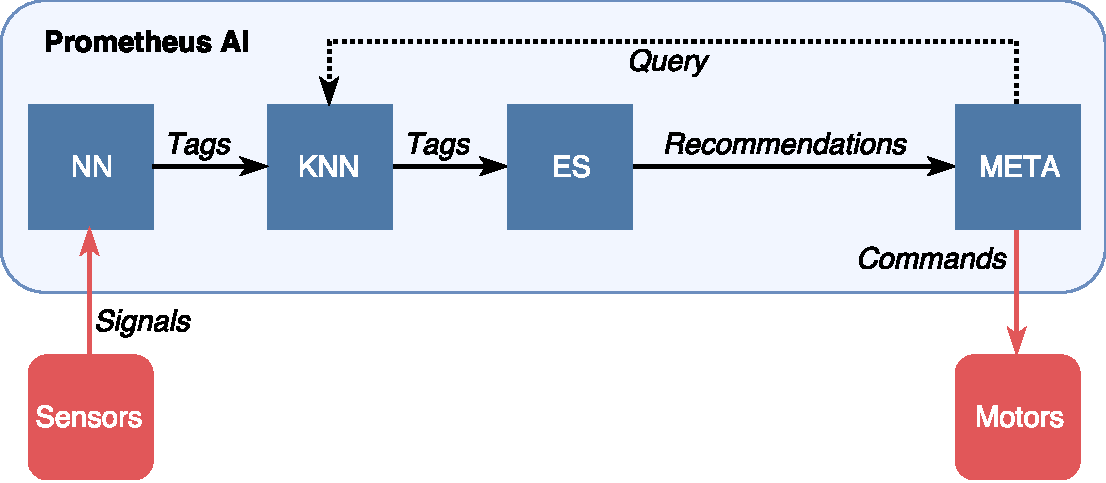
\includegraphics[width=0.99\textwidth]{figures/ai_model_labeled.pdf}
						\caption{Prometheus AI model with labeled input and output.}
						\label{model_labeled}
					\end{figure}
				
					\parbox{0.99\textwidth}{The \textbf{Knowledge Node Network} layer is the analog to memory in the human brain. It takes in the tags provided by the NN and outputs tags based on its knowledge of the environment. It consists of interconnected \textbf{Knowledge Nodes} (KNs), which are abstract structures representing memories and their connections to other memories. The KNN has four ways of searching to fire KNs and activate tags: \textbf{direct}, \textbf{forward}, \textbf{backward} and \textbf{lambda}.}
					
					\begin{figure}[!htb]
						\centering
						\begin{subfigure}[!htb]{0.49\columnwidth}
							\centering
							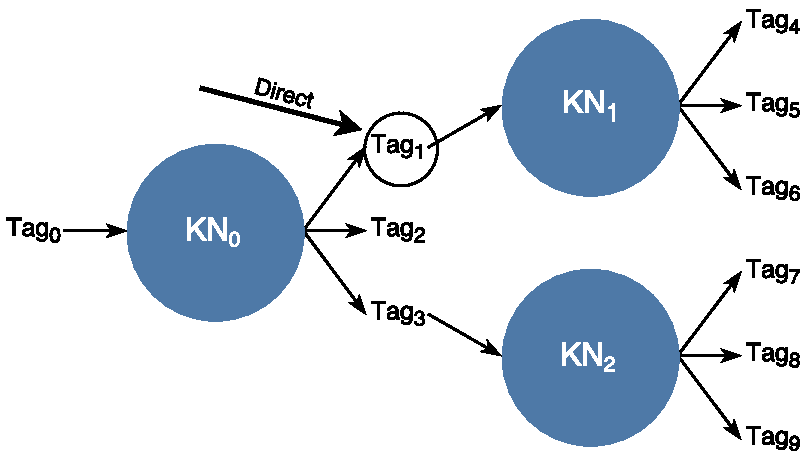
\includegraphics[height=2.8in]{figures/direct_search.pdf}
							\caption{Direct searching.}
						\end{subfigure}
						\begin{subfigure}[!htb]{0.49\columnwidth}
							\centering
							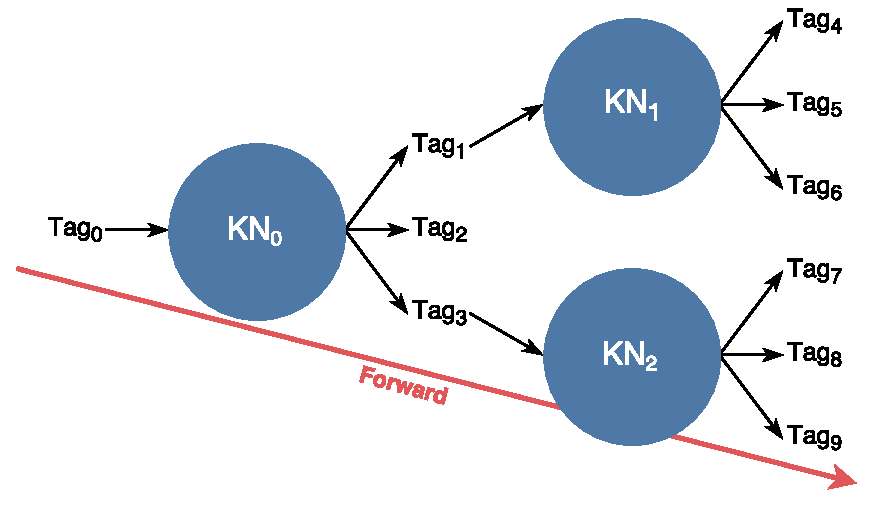
\includegraphics[height=2.8in]{figures/forward_search.pdf}
							\caption{Forward searching/thinking.}
							\label{think_forwards}
						\end{subfigure}
						\bigskip
						\begin{subfigure}[!htb]{0.49\columnwidth}
							\centering
							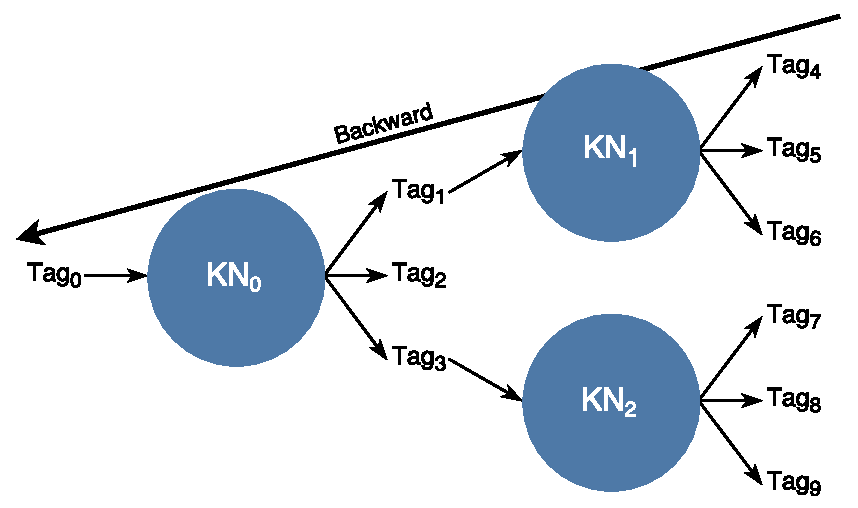
\includegraphics[height=2.8in]{figures/backward_search.pdf}
							\caption{Backward searching/thinking.}
							\label{think_backwards}
						\end{subfigure}
						\begin{subfigure}[!htb]{0.49\columnwidth}
							\centering
							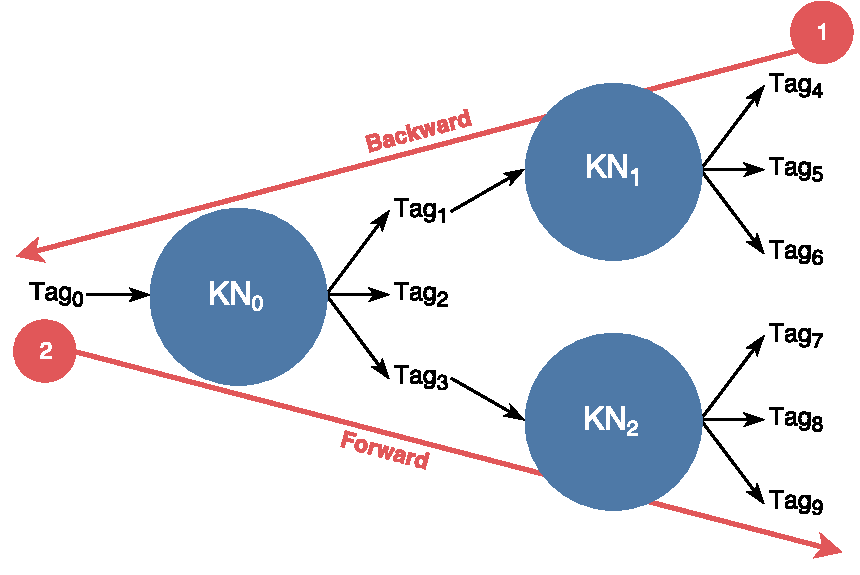
\includegraphics[height=2.8in]{figures/lambda_search.pdf}
							\caption{Lambda searching/thinking.}
							\label{think_lambda}
						\end{subfigure}
						\caption{Methods of searching and thinking in the KNN.}
					\end{figure}
					
					\parbox{0.99\textwidth}{The \textbf{Expert System} layer is a basic logic reasoner. It is not aware of its current reality or any context. It takes in the tags provided by the KNN and interprets them as either \textbf{facts}, \textbf{recommendations} or \textbf{rules}.
						
					\begin{figure}[!htb]
						\centering
						\begin{subfigure}[!htb]{0.4\columnwidth}
							\centering
							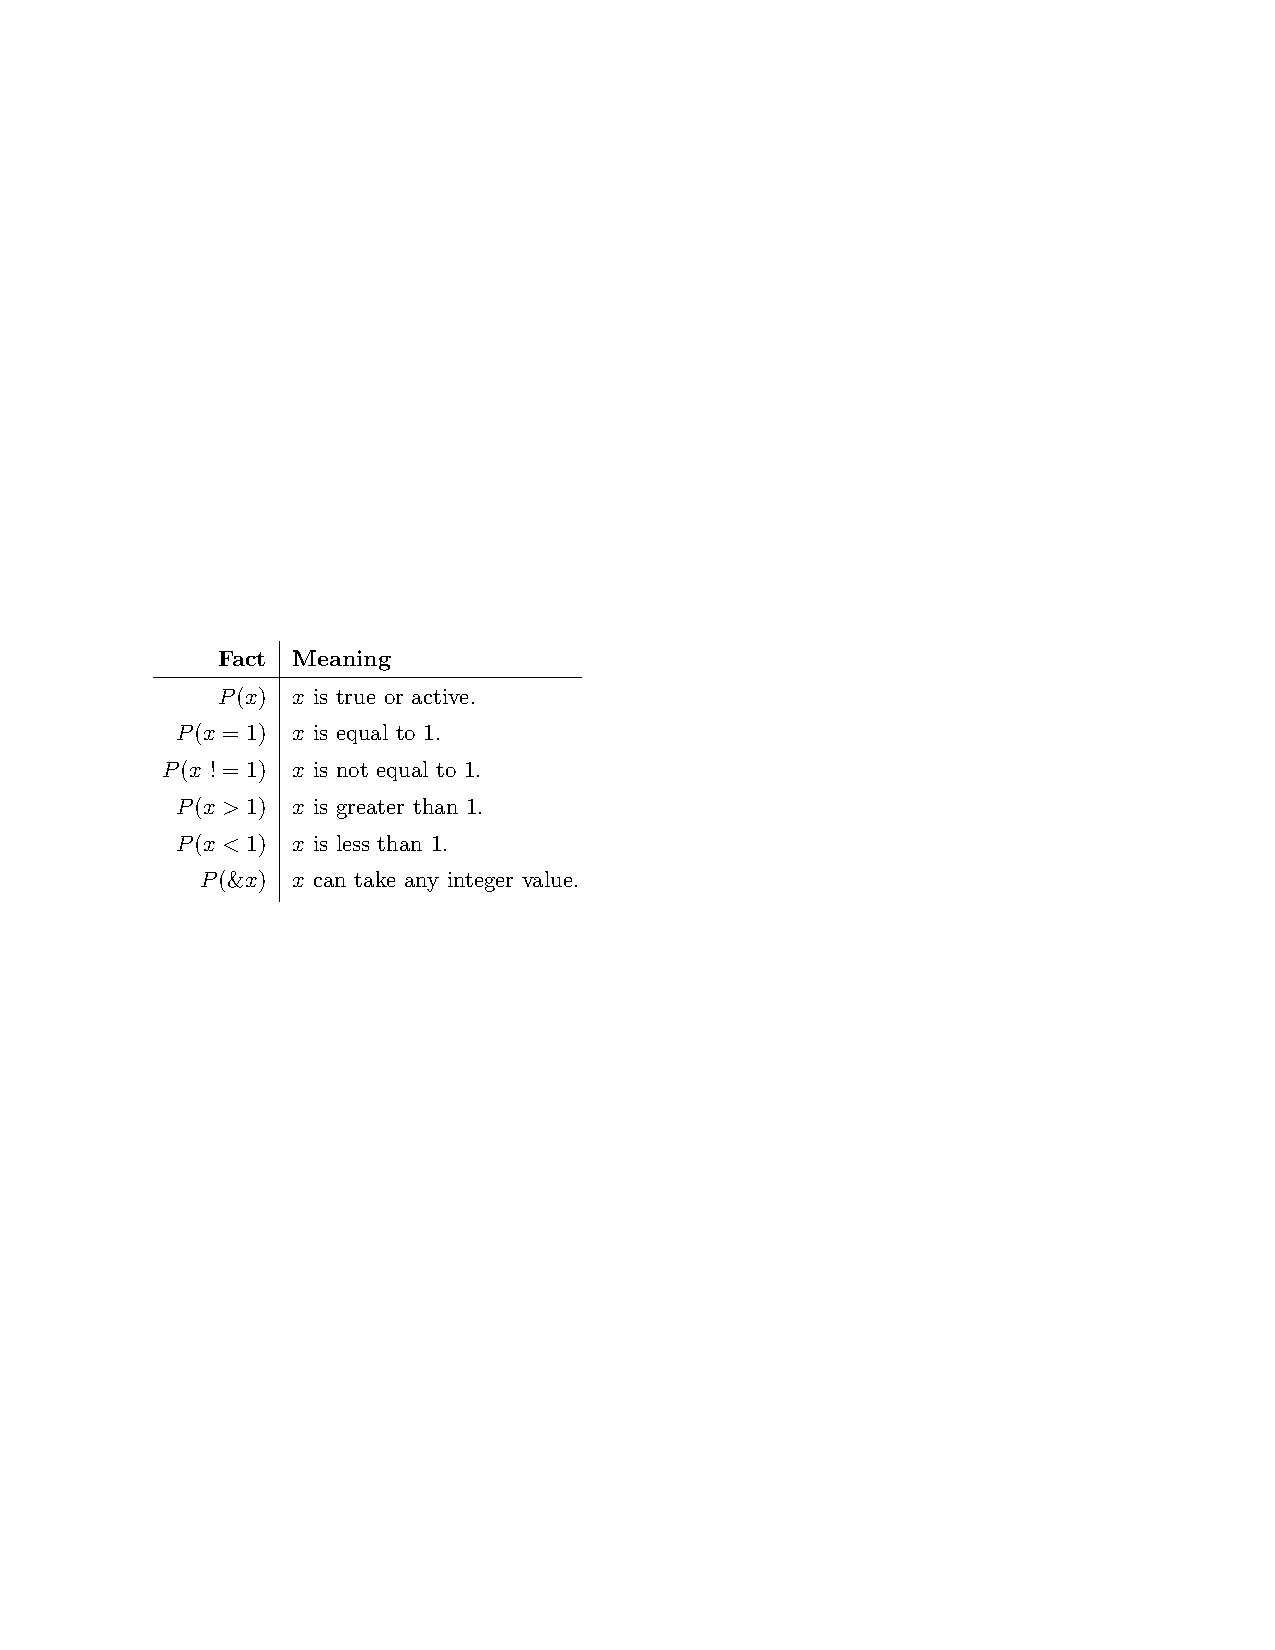
\includegraphics[height=2in]{figures/fact_examples.pdf}
							\caption{Examples of simple facts in the ES.}
						\end{subfigure}
						\begin{subfigure}[!htb]{0.58\columnwidth}
							\centering
							
\includegraphics[width=0.5\columnwidth]{figures/fact.pdf}
							\caption{The form of a fact in the ES. $P$ is a predicate, and $A_i$ is an argument.}
							
							\vspace{2ex}
							
							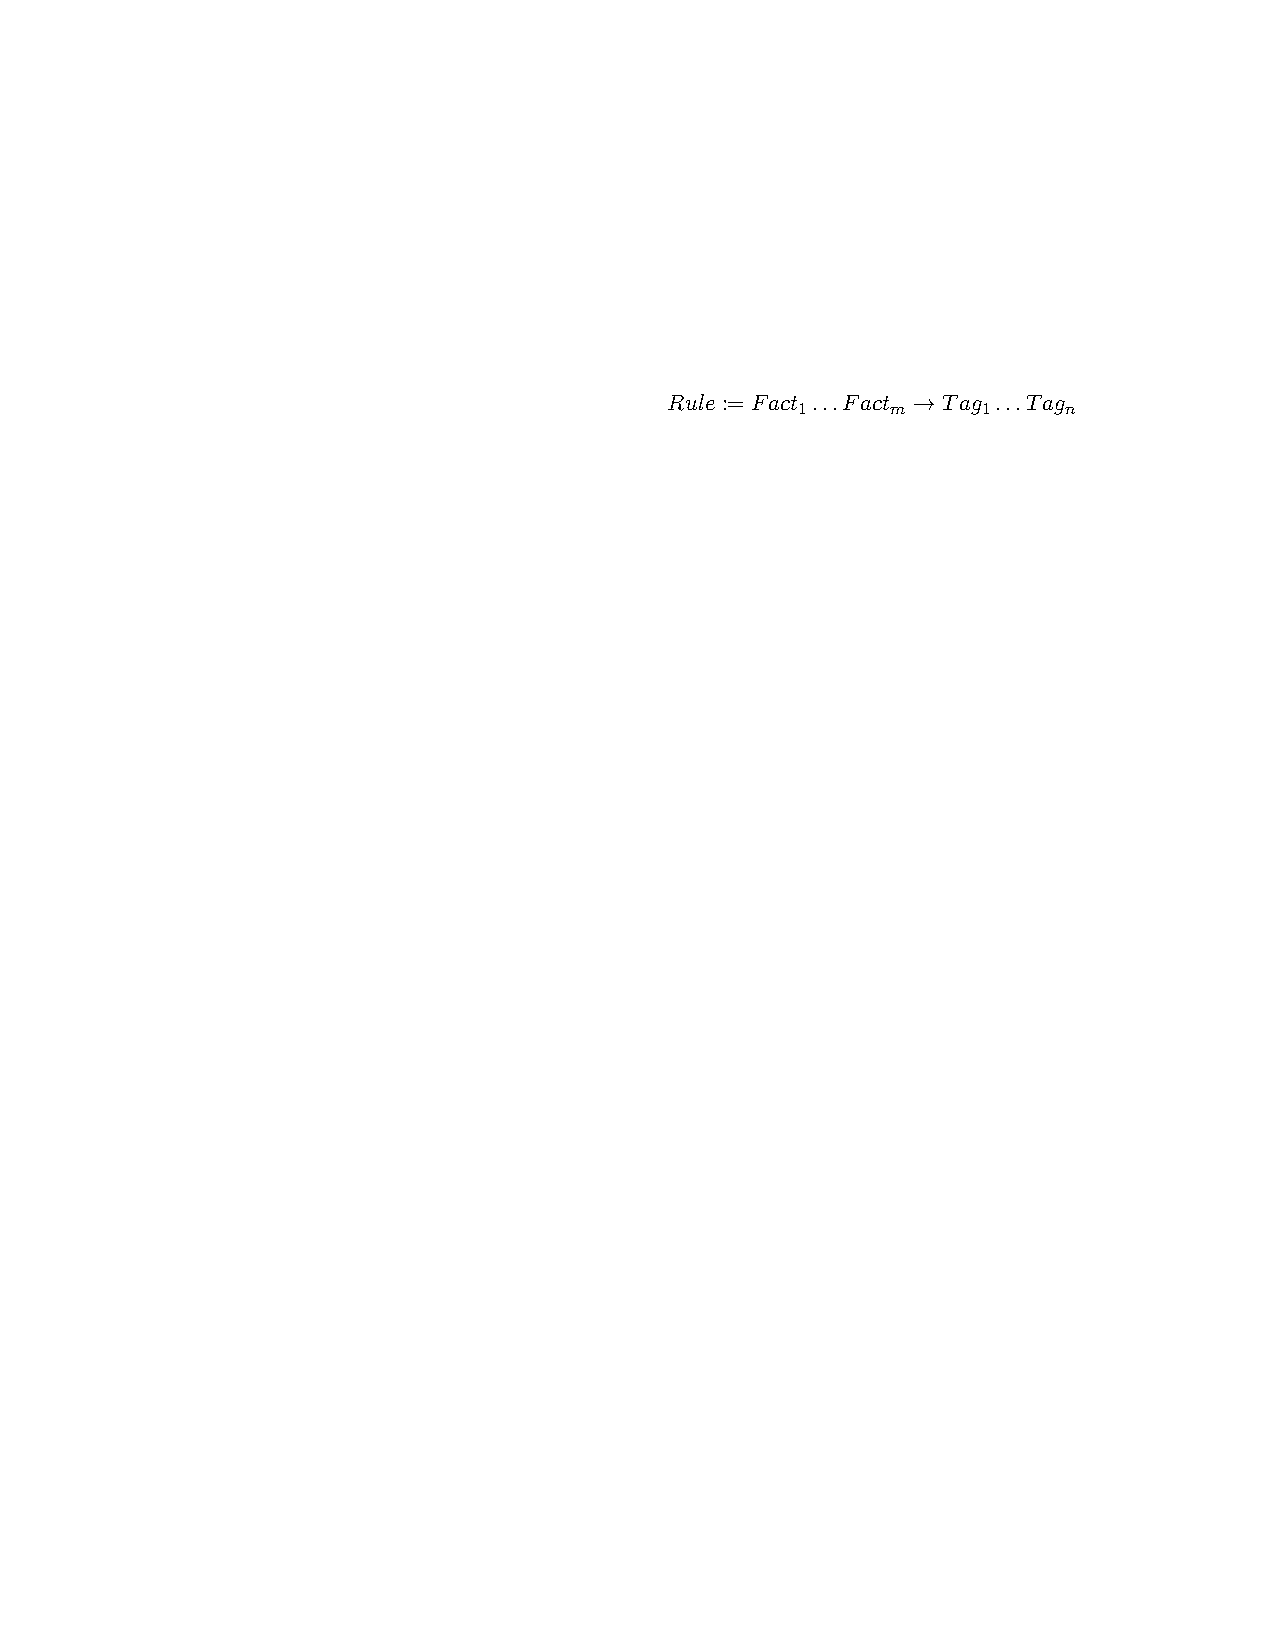
\includegraphics[width=\columnwidth]{figures/rule.pdf}
							\caption{The form of a rule in the ES, with $m$ input facts and $n$ output tags.}
						\end{subfigure}
						\caption{Facts and Rules in the ES.}
					\end{figure}
					
					
					The \textbf{Meta Reasoner} represents high-level reasoning in the human brain. It is aware of its environment and context, and makes decisions based on what it believes to be right.}
				\end{block}
			}
			\end{column}
			\begin{column}{.33\textwidth}
				\parbox[t][\columnheight]{\textwidth}{
				
				\begin{block}{Problem}
					There are two main assigned tasks over the past two semesters:
					\begin{enumerate}
						\item Design and implement the \textbf{Expert System} and \textbf{Knowledge Node Network} in Java.
						\begin{itemize}
							\item Create an initial design.
							\item Build a code skeleton.
							\item Implement integration and unit tests.
						\end{itemize}
						
						\item Supervise undergraduate students working on Prometheus.
						\begin{itemize}
							\item Provide resources.
							\item Review code.
						\end{itemize}
					\end{enumerate}
				\end{block}
					
				\begin{block}{Design \& Implementation}
%					\begin{itemize}
%						\item Dependencies modeled using Google Guice.
%						\begin{itemize}
%							\item Framework for modular dependency injection.
%							\item Allows for easily testable code.
%						\end{itemize}
%					\end{itemize}
					
					\parbox{0.99\textwidth}{The \textbf{tags} are implemented using a \code{Tag} Java class, with \code{Predicate} and \code{Rule} subclasses. The \code{Predicate} class is a superclass of the \code{Fact} and \code{Recommendation}. Searching in the \textbf{Knowledge Node Network} is implemented by \code{directSearch()}, \code{forwardSearch()}, \code{backwardSearch()} and \code{lambdaSearch()}.}
				
					\begin{figure}
						\centering
						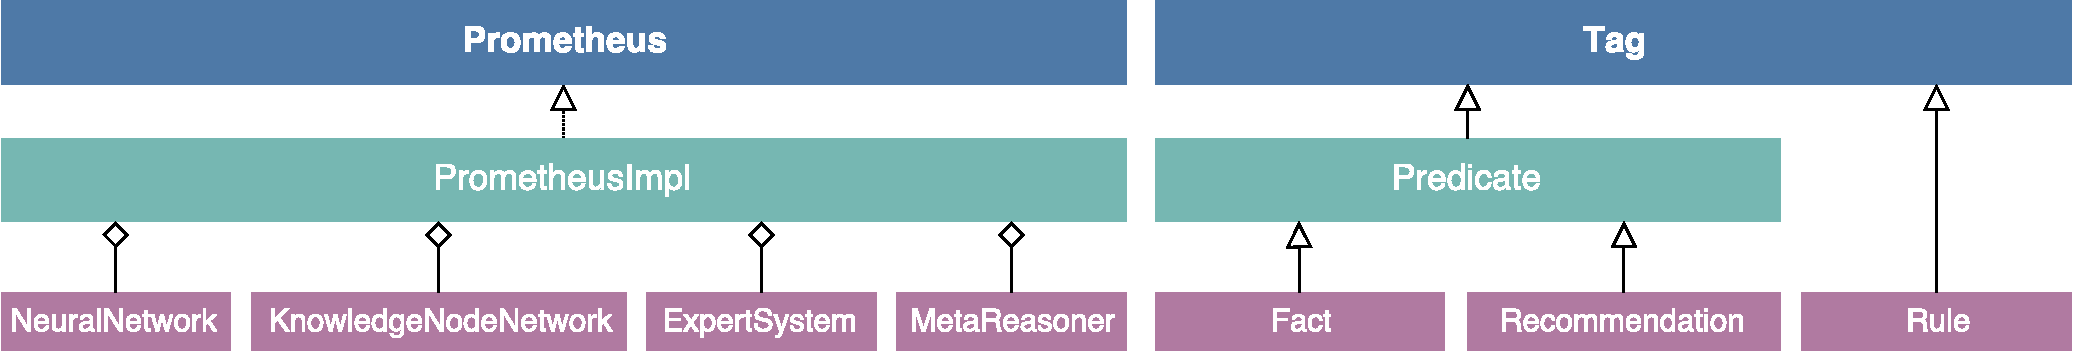
\includegraphics[width=0.99\textwidth]{figures/uml_combined_1.pdf}
						\caption{UML diagrams of the Prometheus and Tag packages.}
					\end{figure}			
				
					\parbox{0.99\textwidth}{
					The most important method in the \textbf{Expert System} is \code{think()}, which executes thinking cycles and output recommendations.}
				
					\begin{figure}
						\centering
						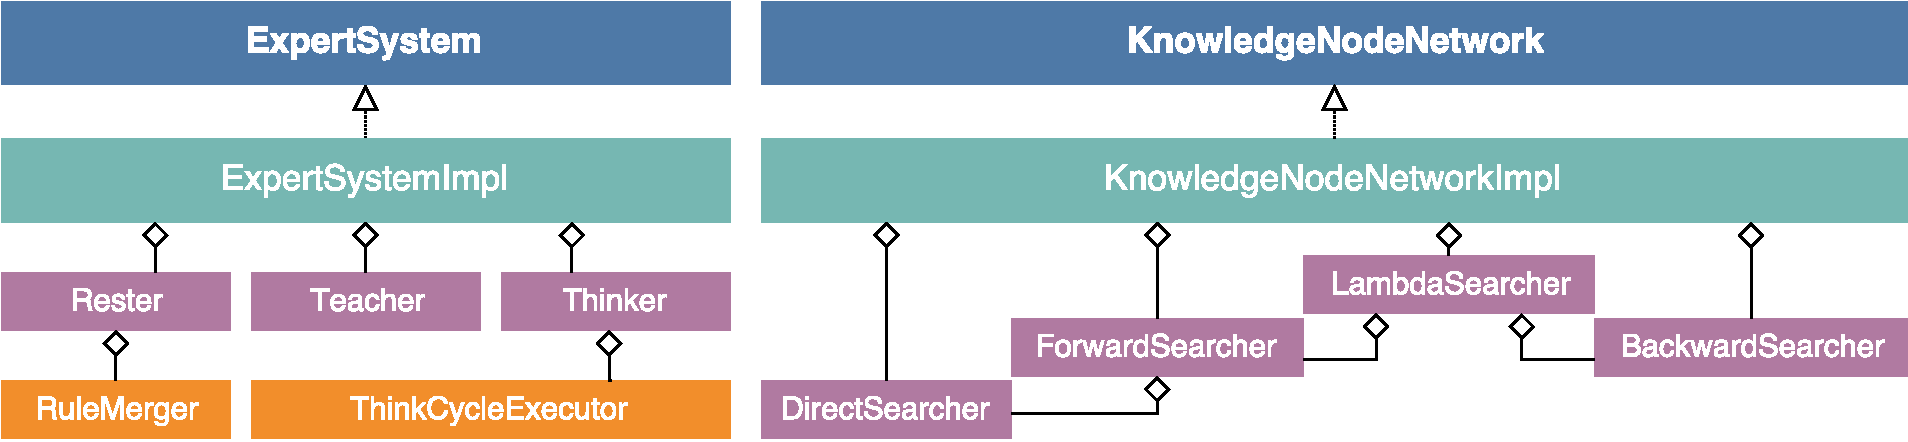
\includegraphics[width=0.99\textwidth]{figures/uml_combined_3.pdf}
						\caption{UML diagrams of Expert System and Knowledge Node Network packages.}
					\end{figure}
				
					\parbox{0.99\textwidth}{
					The Java \textbf{graph visualization} library GraphStream was used to visualize the KNN and the process of searching or thinking through it.}
				
					\begin{figure}
						\centering
						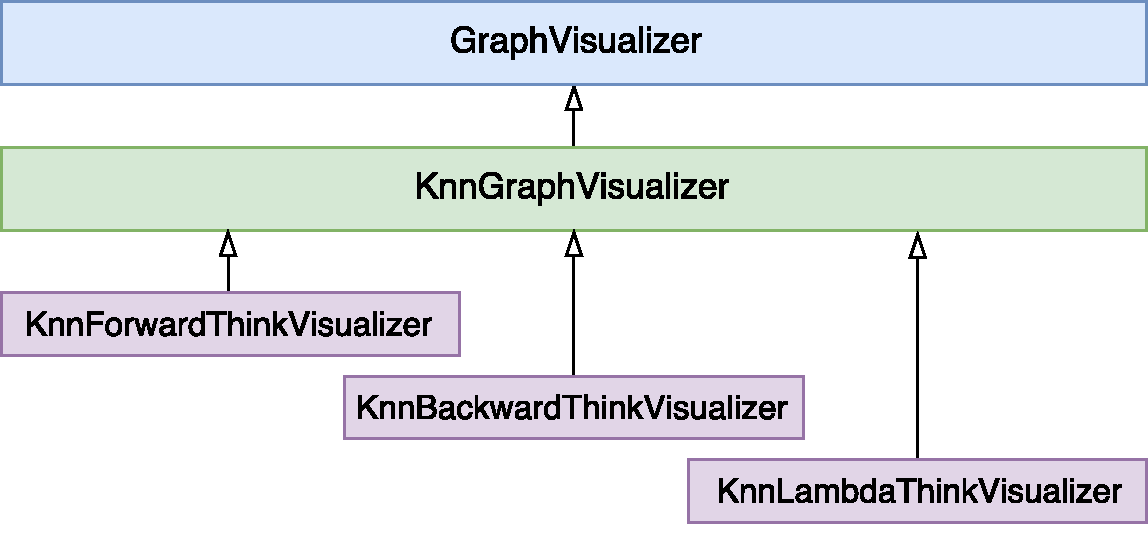
\includegraphics[width=0.55\textwidth]{figures/uml_graphing.pdf}
						\caption{UML diagrams of the graphing package.}
					\end{figure}
					
					\begin{figure}[!htb]
						\centering
						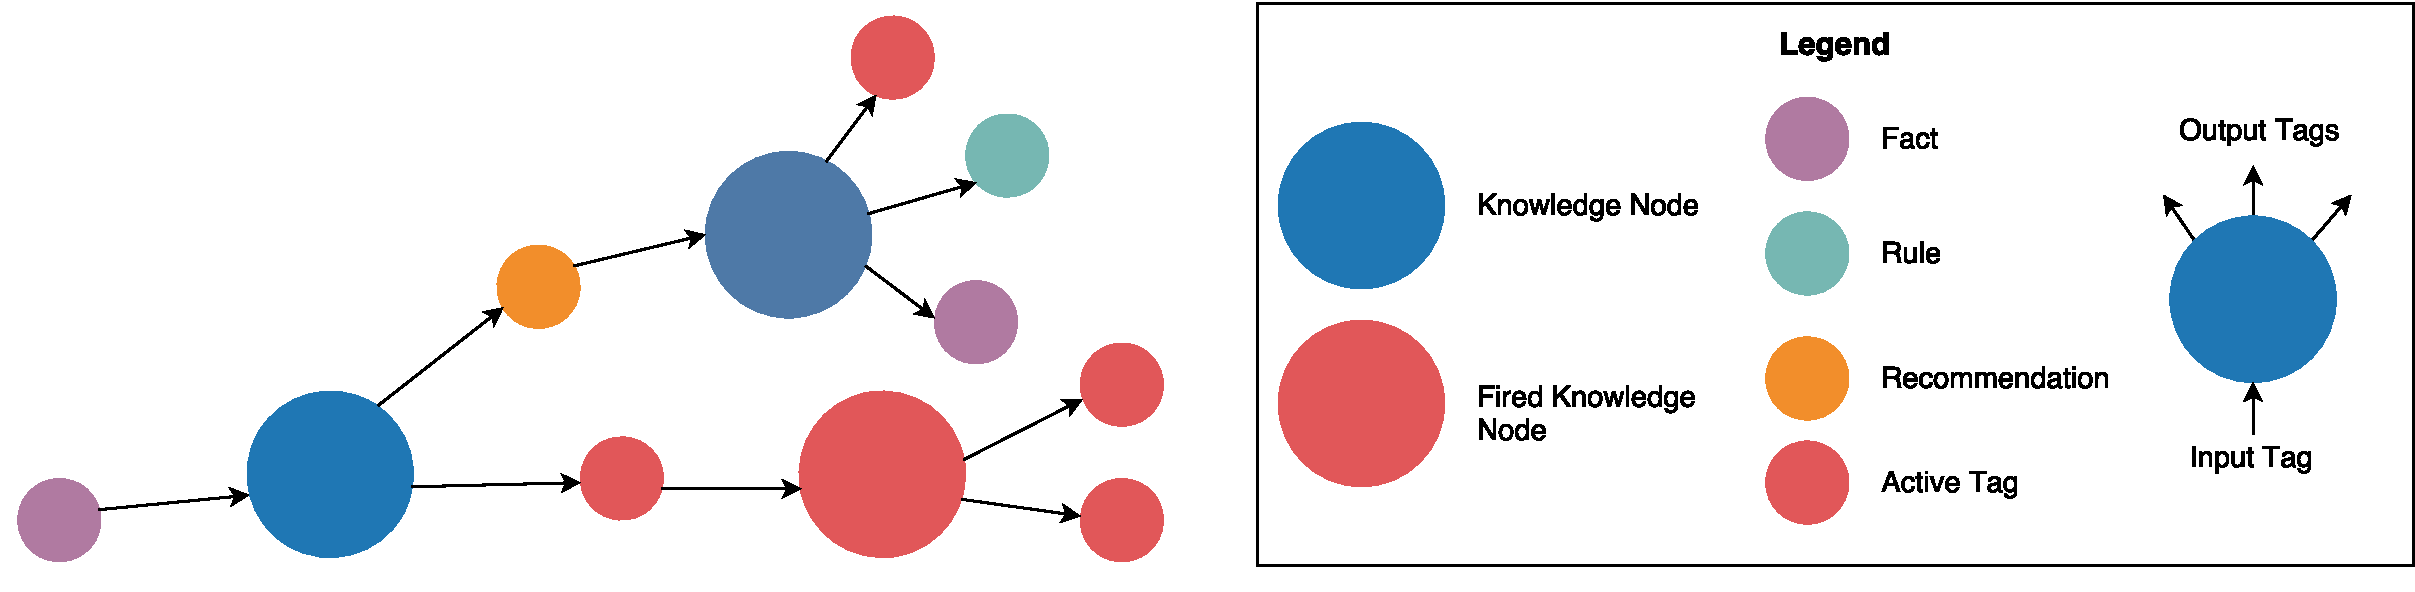
\includegraphics[width=\columnwidth]{figures/knn_graph_legend.pdf}
						\caption
						{Legend for the visualization of the KNN.}
					\end{figure}
					
				\end{block}
				}
			\end{column}
			\begin{column}{.33\textwidth}
				\parbox[t][\columnheight]{\textwidth}{
				\begin{block}{Results \& Tests}
					\parbox{0.99\textwidth}{
						\textbf{Unit tests} were created using \textbf{Mockito}, \textbf{TestNG} and \textbf{TestNG}. These tests test the functionality of isolated methods. \textbf{Integration tests} were also created with \textbf{TestNG}, testing end-to-end behavior.}
					
					\begin{figure}[!htb]
						\centering
						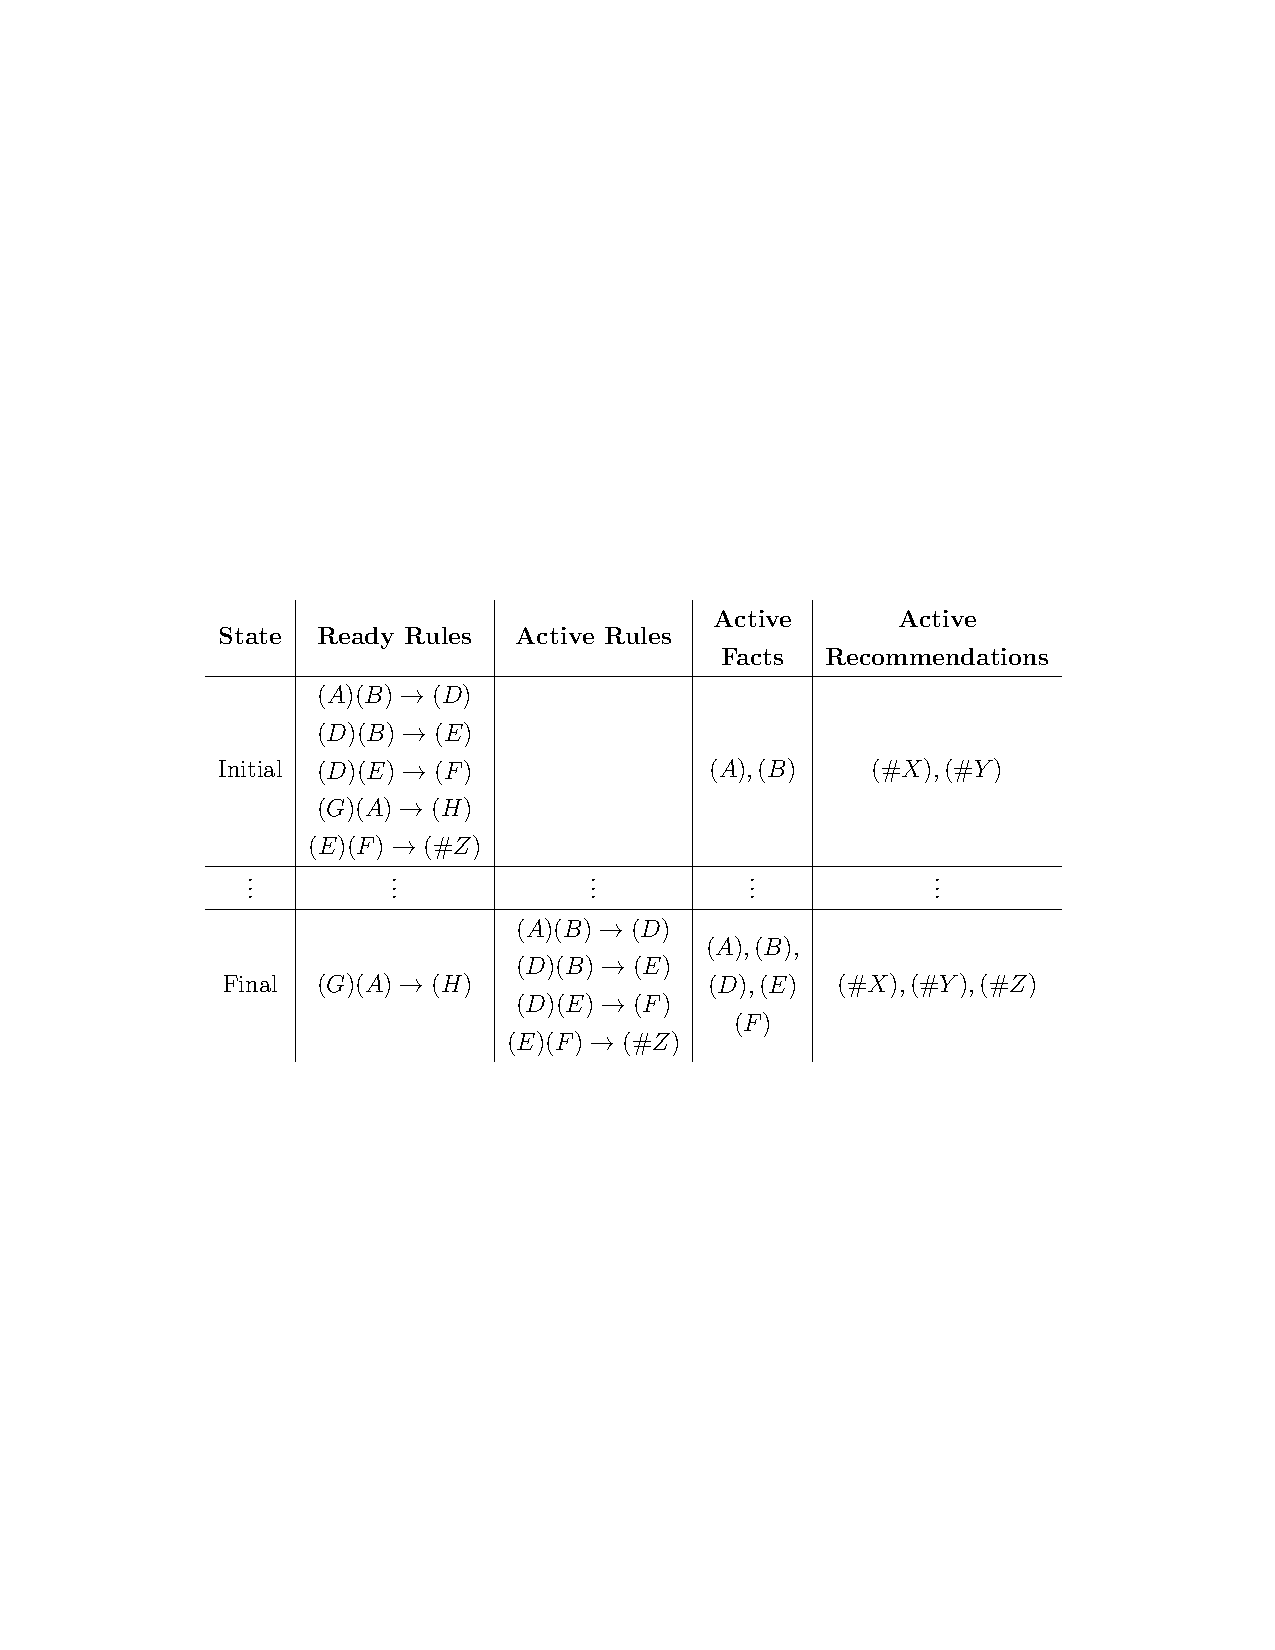
\includegraphics[width=0.7\textwidth]{figures/testES.pdf}
						\caption
						{ES test setup representing simple rules and facts that must be brought to quiescence.}
					\end{figure}
%					\begin{figure}[!htb]
%						\centering
%						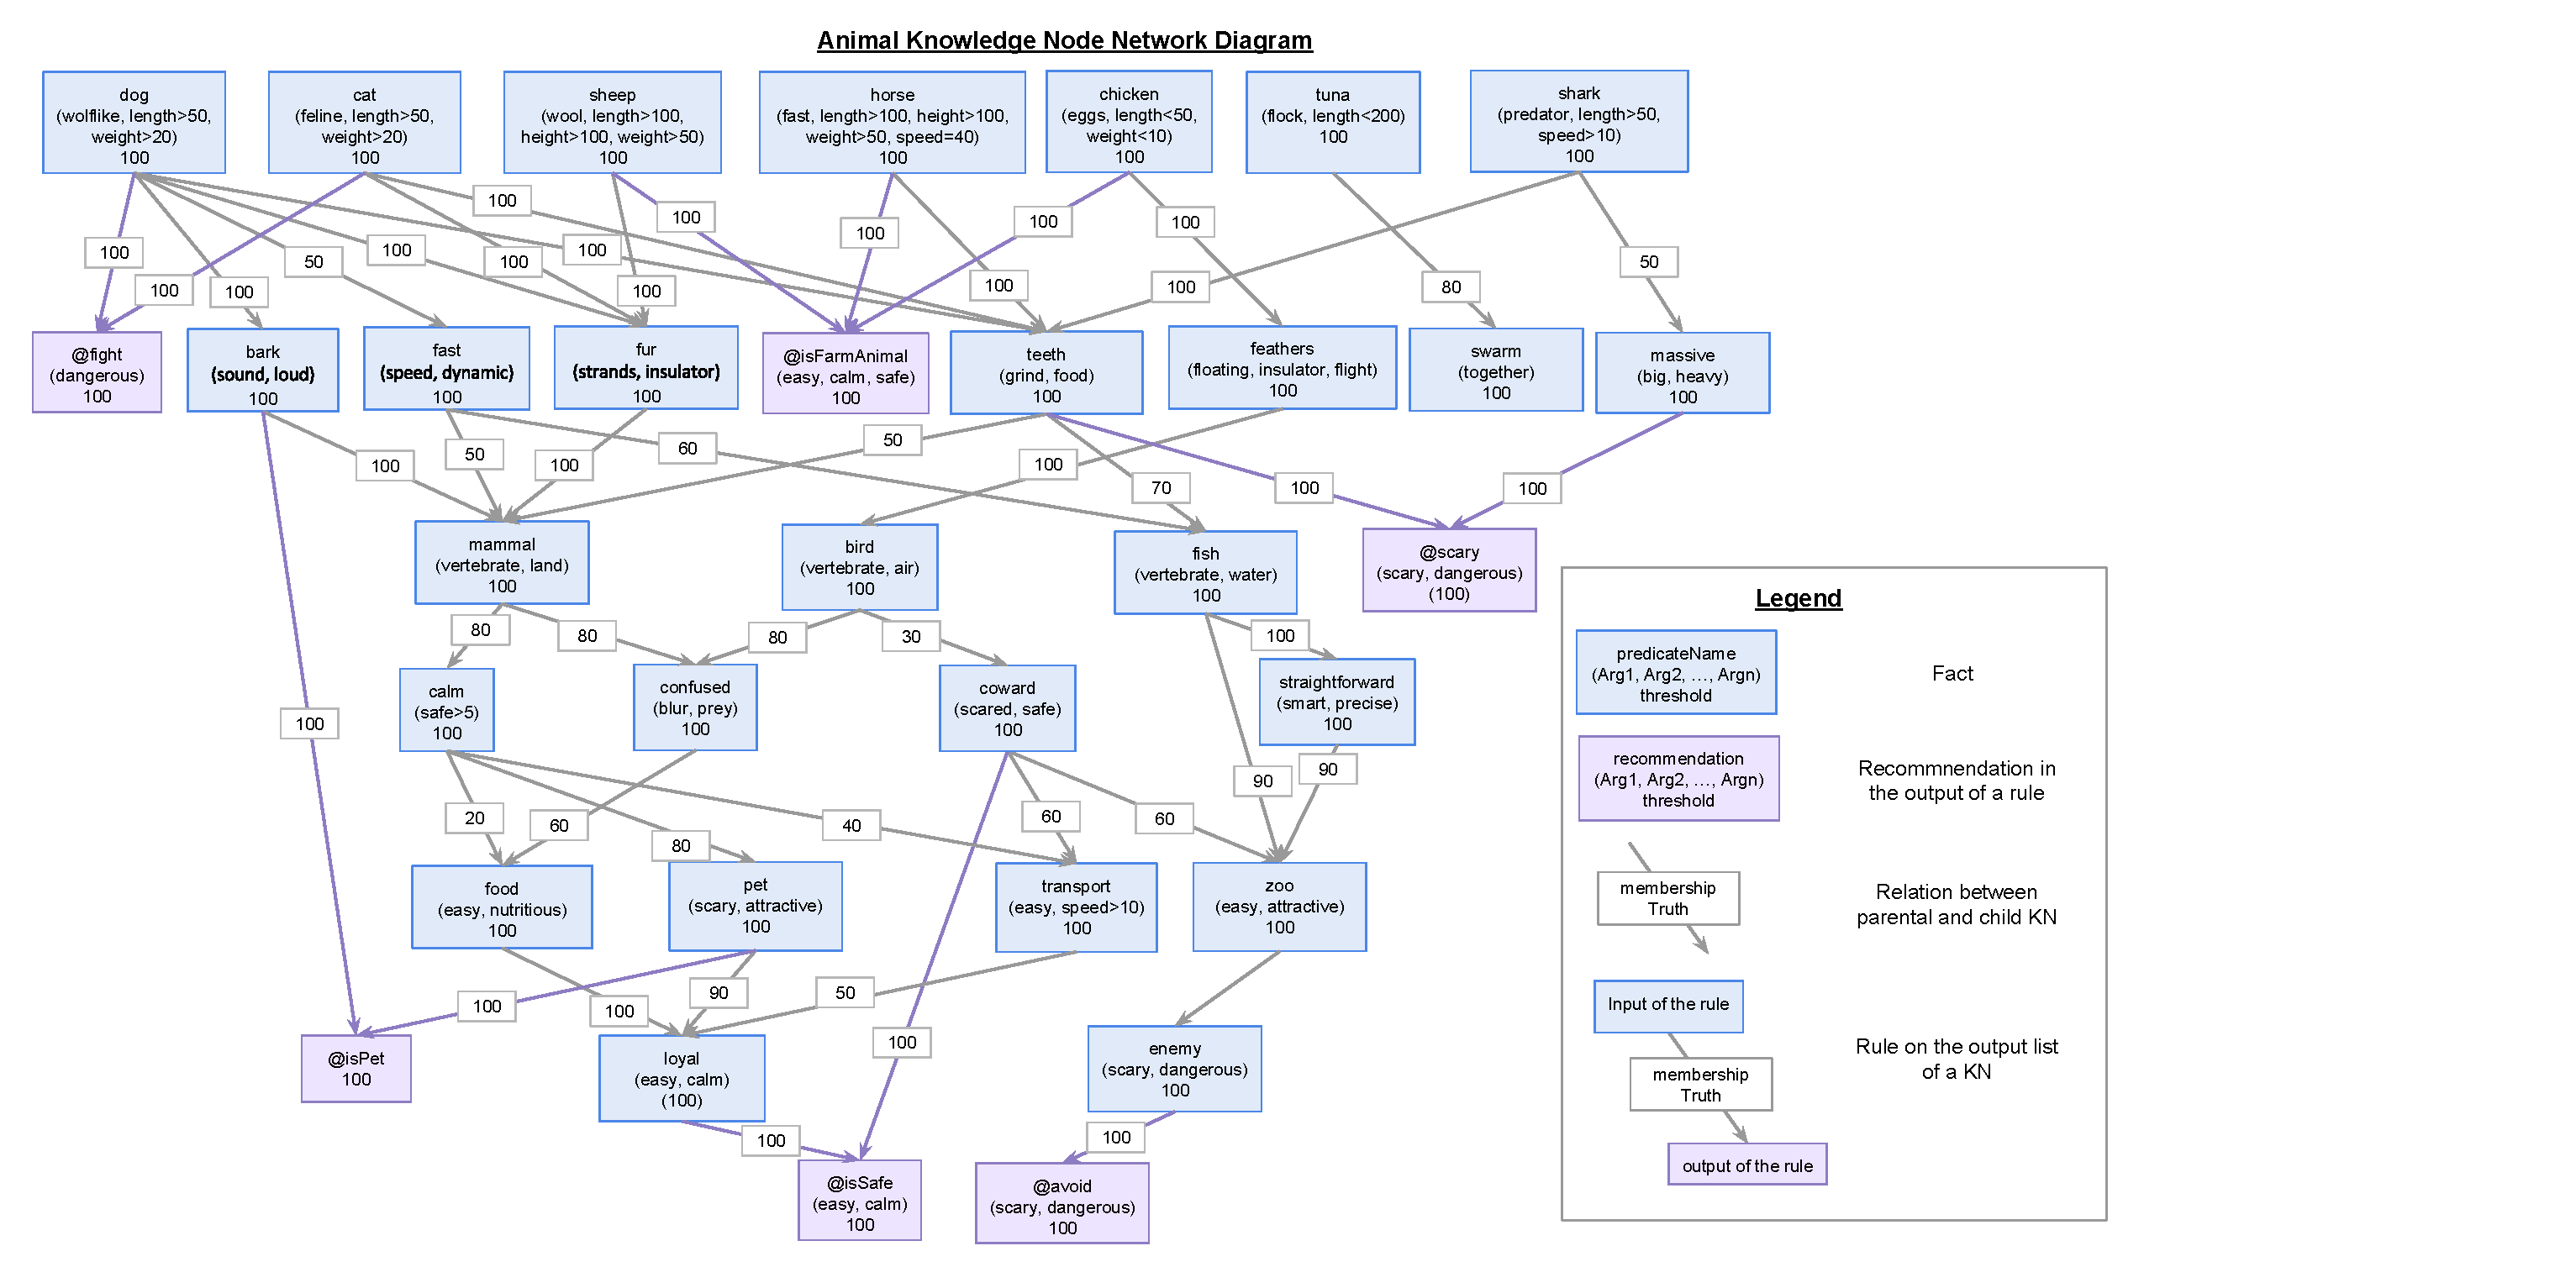
\includegraphics[width=\textwidth]{figures/animal_knn.pdf}
%						\caption
%						{Elaborate test KNN network representing connections between memories of animals and their characteristics. Credit for creating the graph goes to volunteer Laurence Liang.}
%					\end{figure}
					
					\begin{itemize}
						\item Graph visualization tests.
						\begin{itemize}
							\item Iterations of the KNN searching algorithms are presented visually.
							\item Small nodes are Tags, big nodes are Knowledge Nodes (KNs).
							\item Red nodes represent active Tags or fired KNs. 
							\item For non-active Tags, Facts are purple, Rules are blue and Recommendations are orange.
						\end{itemize}
					\end{itemize}
					
					\begin{figure}[!htb]
						\centering
						\begin{subfigure}[!htb]{0.32\columnwidth}
							\centering
							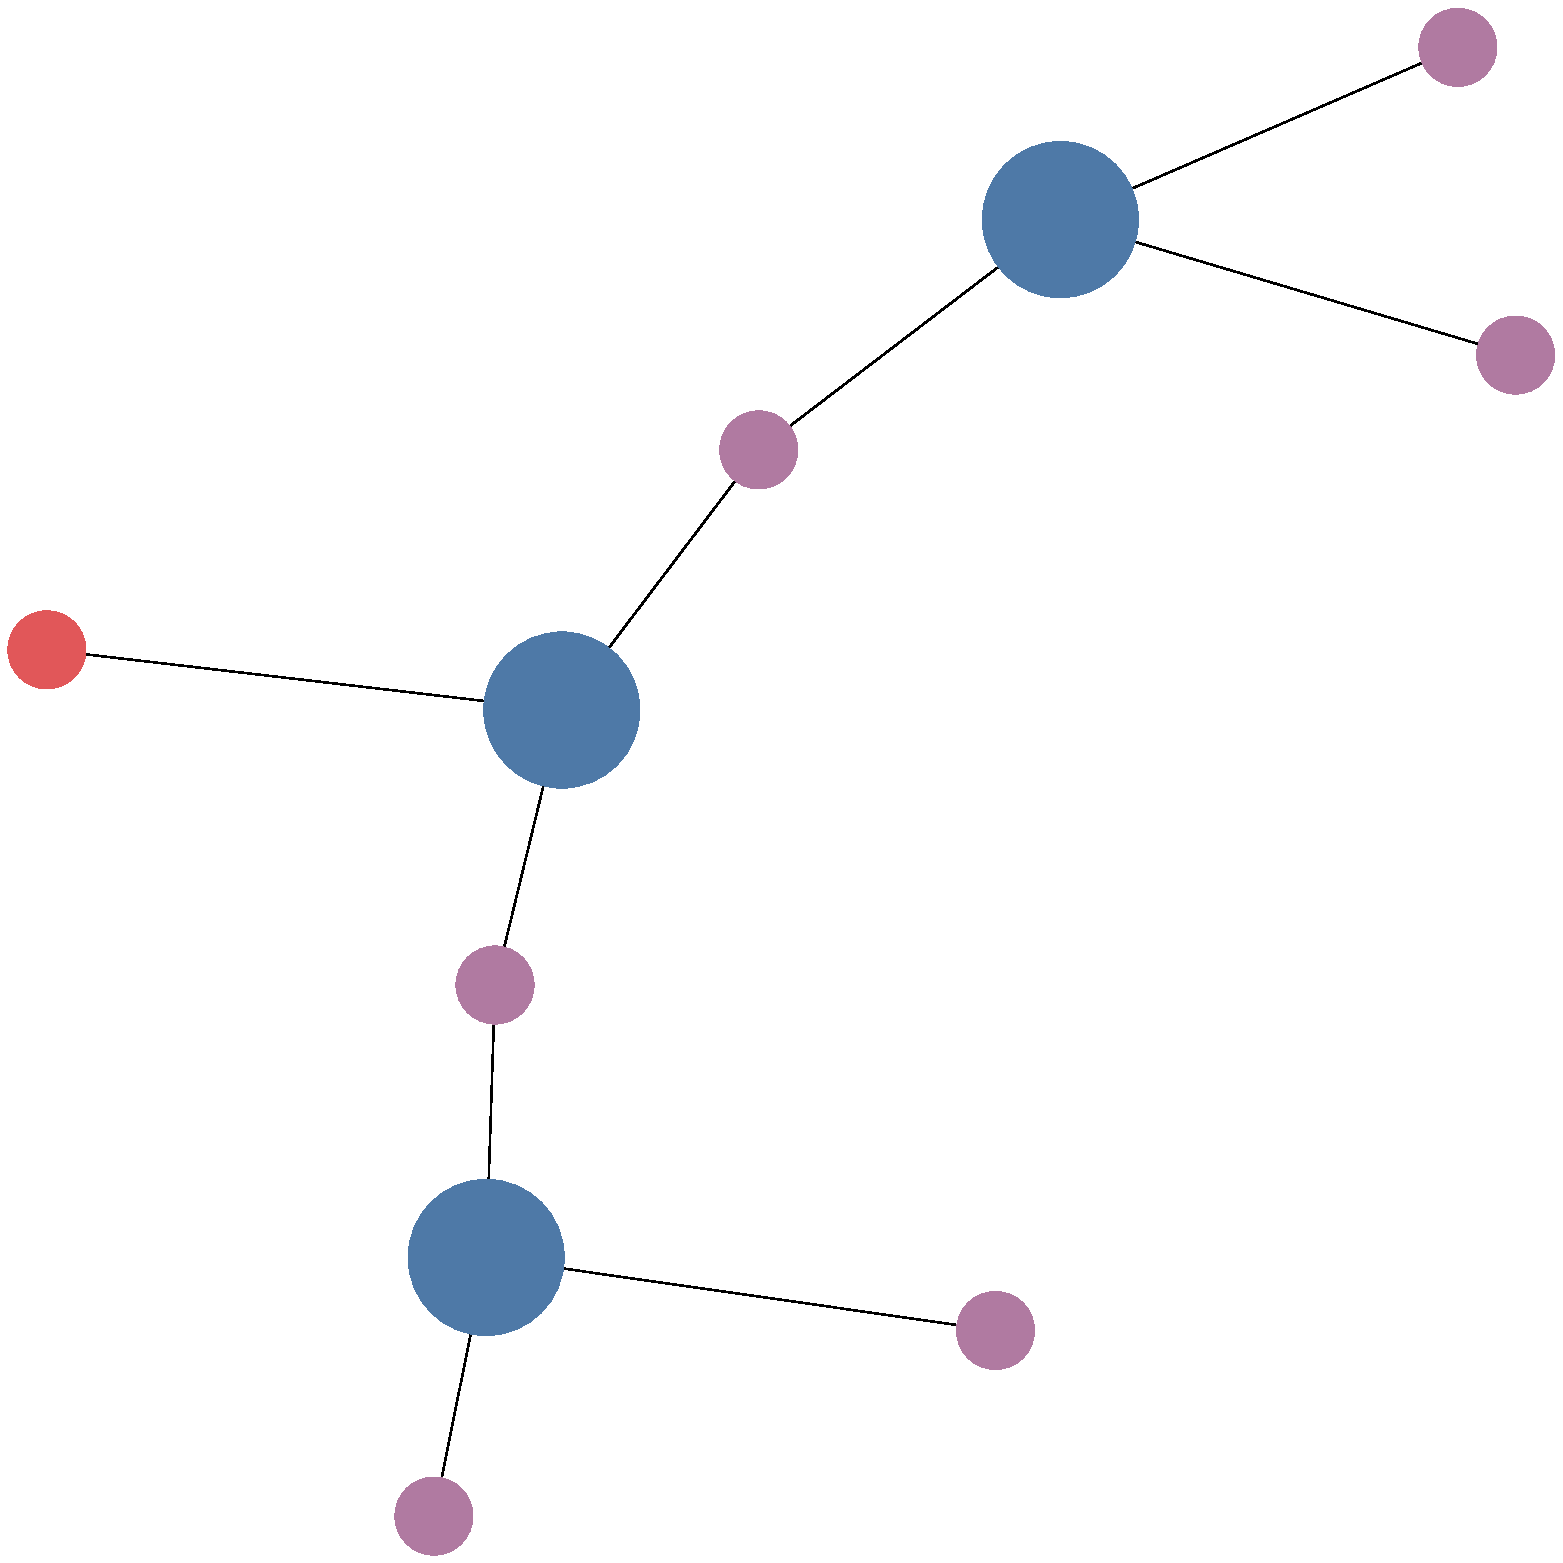
\includegraphics[width=\columnwidth]{figures/knn_simple_forward_think_0.pdf}
							\caption{Ply 1.}
						\end{subfigure}
						\begin{subfigure}[!htb]{0.32\columnwidth}
							\centering
							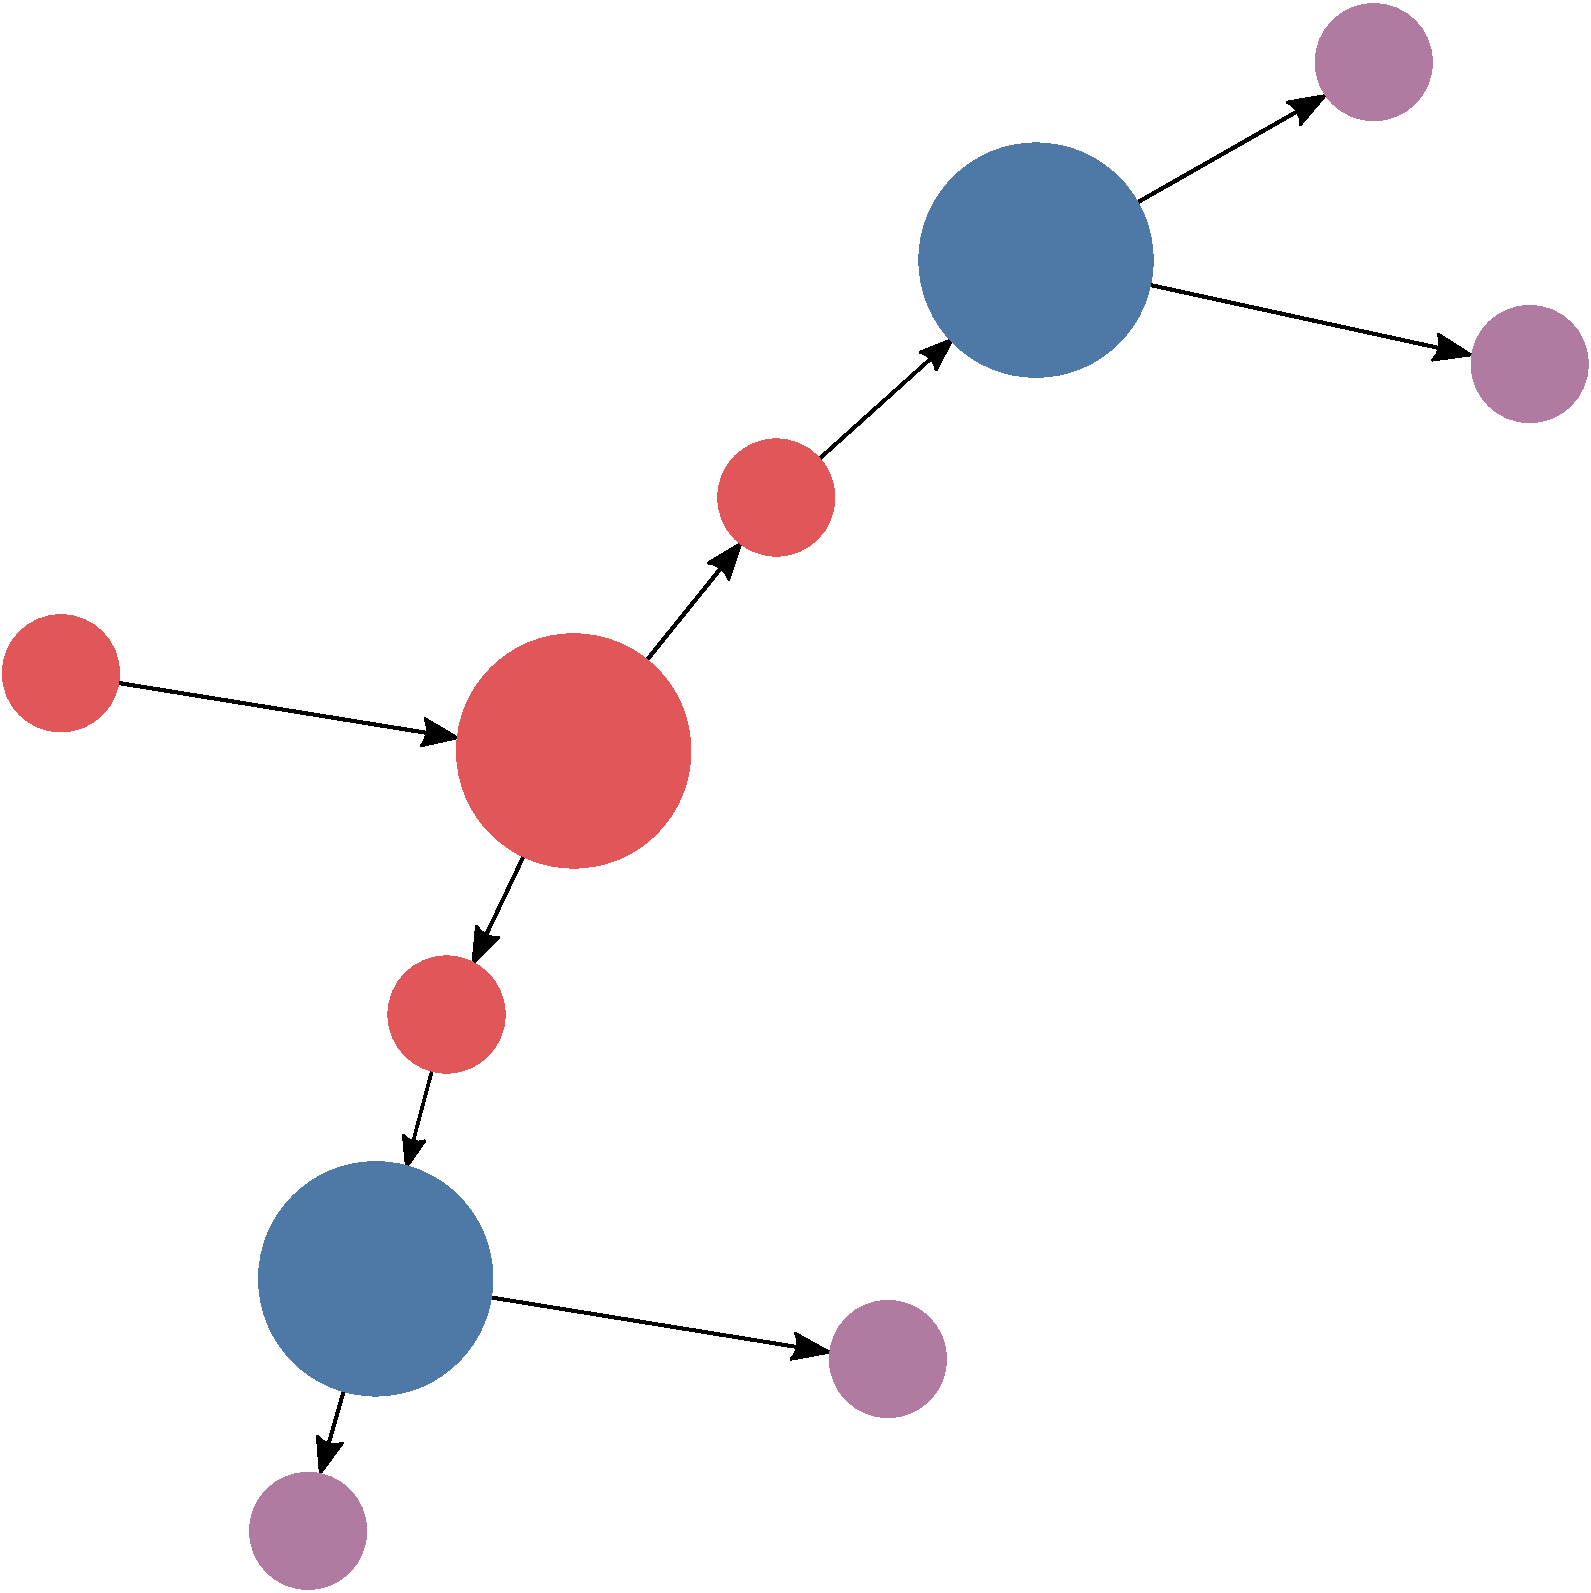
\includegraphics[width=\columnwidth]{figures/knn_simple_forward_think_1.pdf}
							\caption{Ply 2.}
						\end{subfigure}
						\begin{subfigure}[!htb]{0.32\columnwidth}
							\centering
							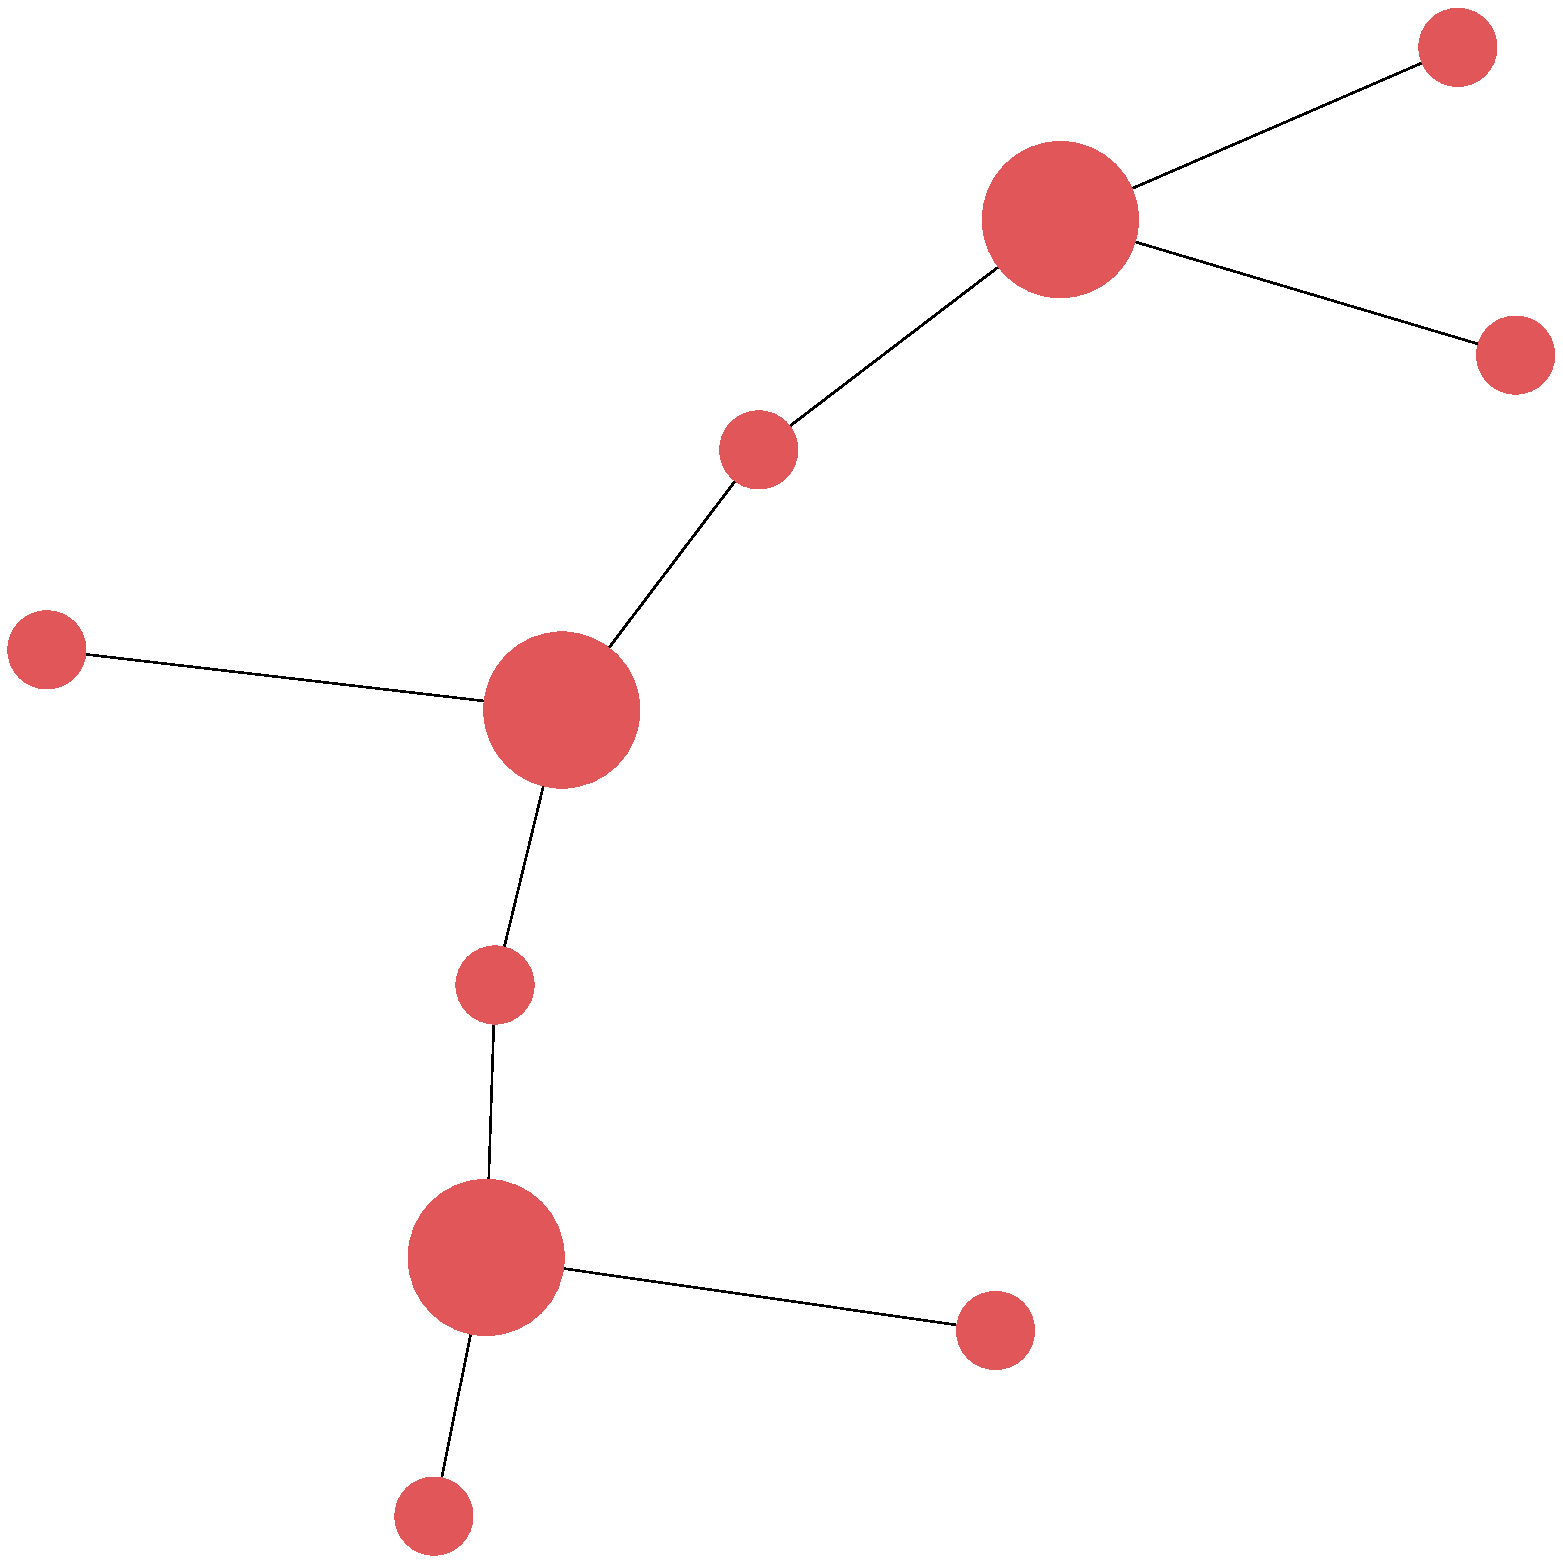
\includegraphics[width=\columnwidth]{figures/knn_simple_forward_think_2.pdf}
							\caption{Ply 3.}
						\end{subfigure}
						\caption{Forward thinking visualization in the KNN.}
					\end{figure}
					
					\begin{figure}[!htb]
						\centering
						\begin{subfigure}[!htb]{0.32\columnwidth}
							\centering
							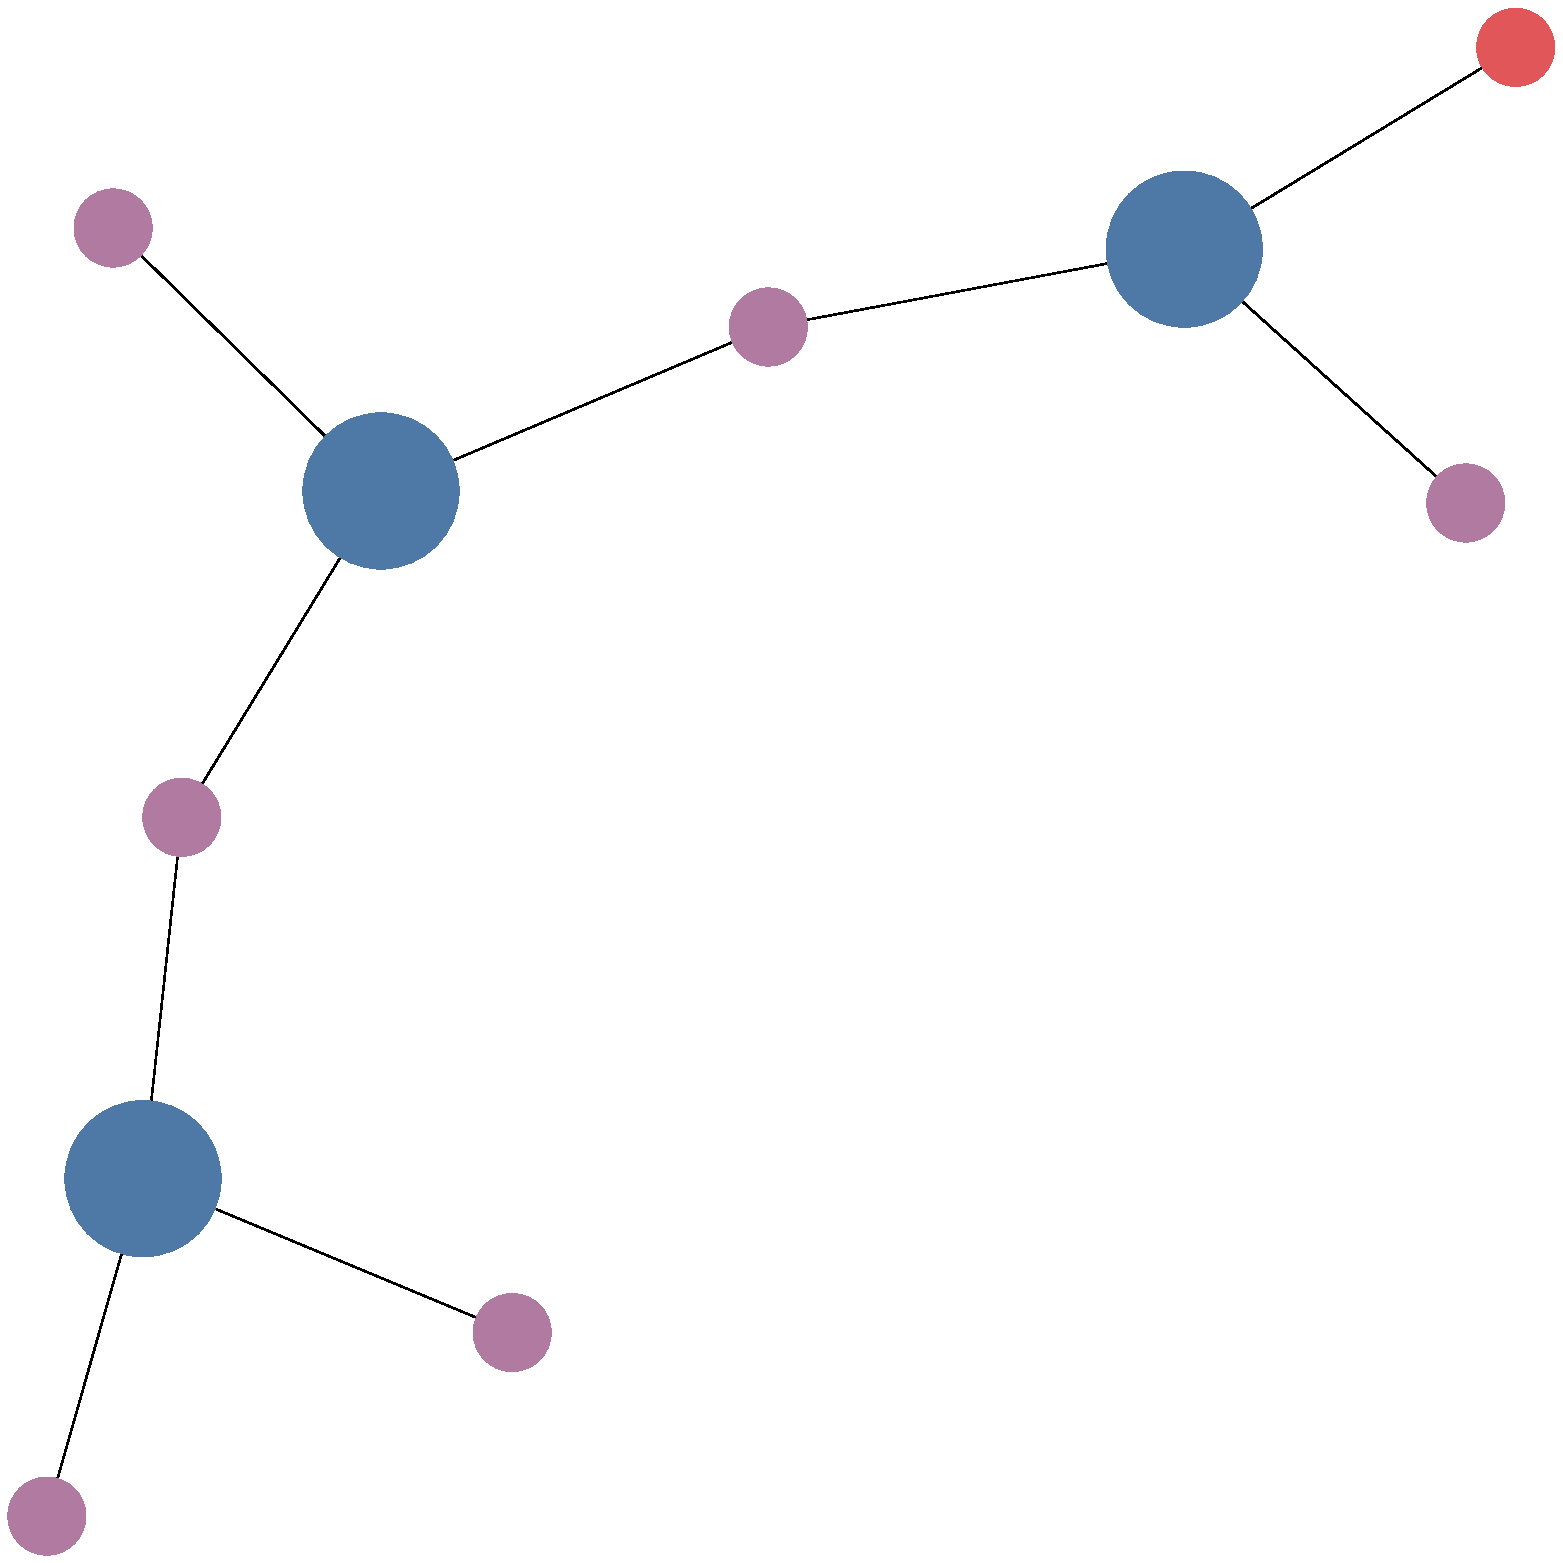
\includegraphics[width=\columnwidth]{figures/knn_simple_backward_think_0.pdf}
							\caption{Ply 1.}
						\end{subfigure}
						\begin{subfigure}[!htb]{0.32\columnwidth}
							\centering
							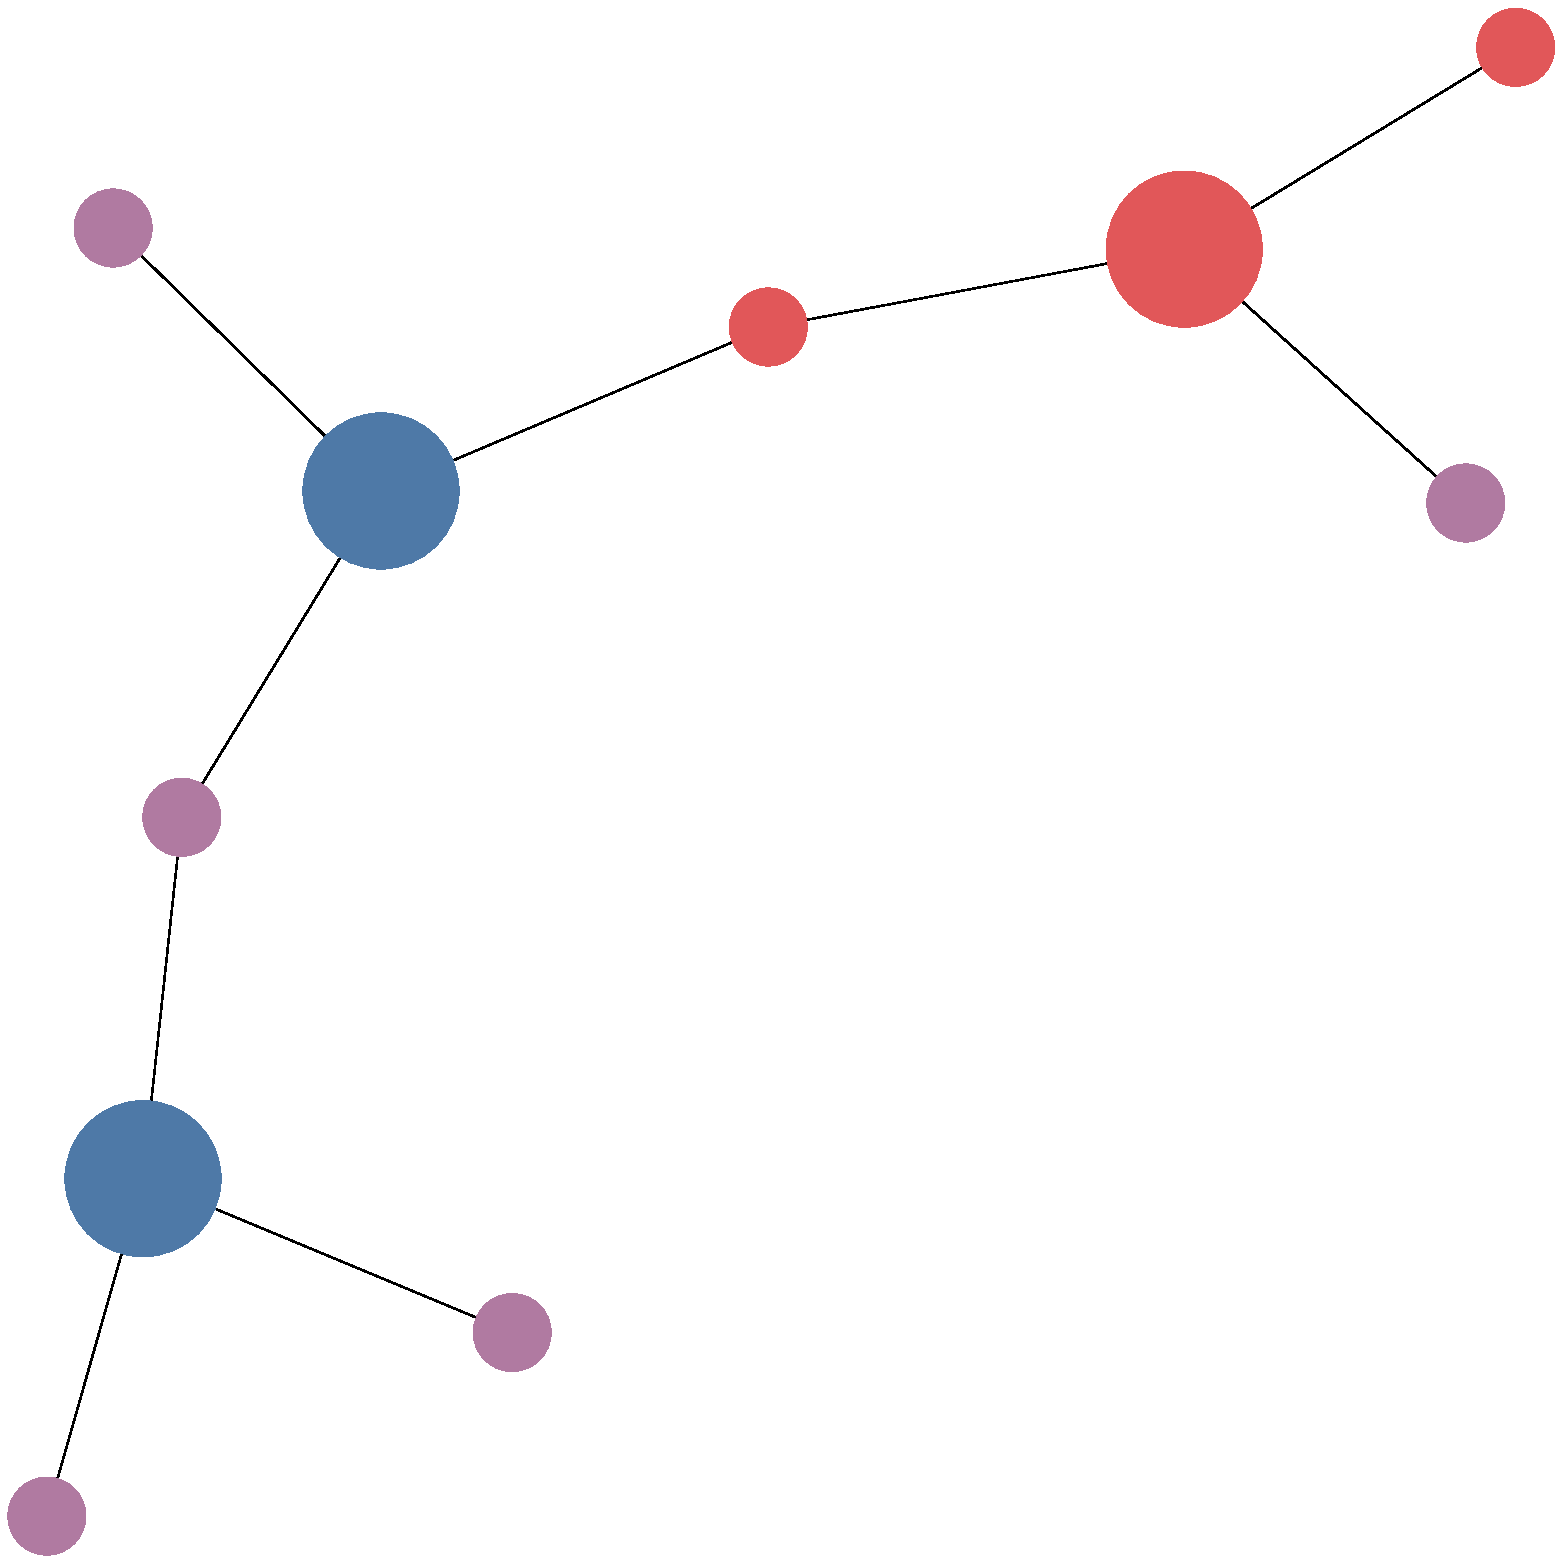
\includegraphics[width=\columnwidth]{figures/knn_simple_backward_think_1.pdf}
							\caption{Ply 2.}
						\end{subfigure}
						\begin{subfigure}[!htb]{0.32\columnwidth}
							\centering
							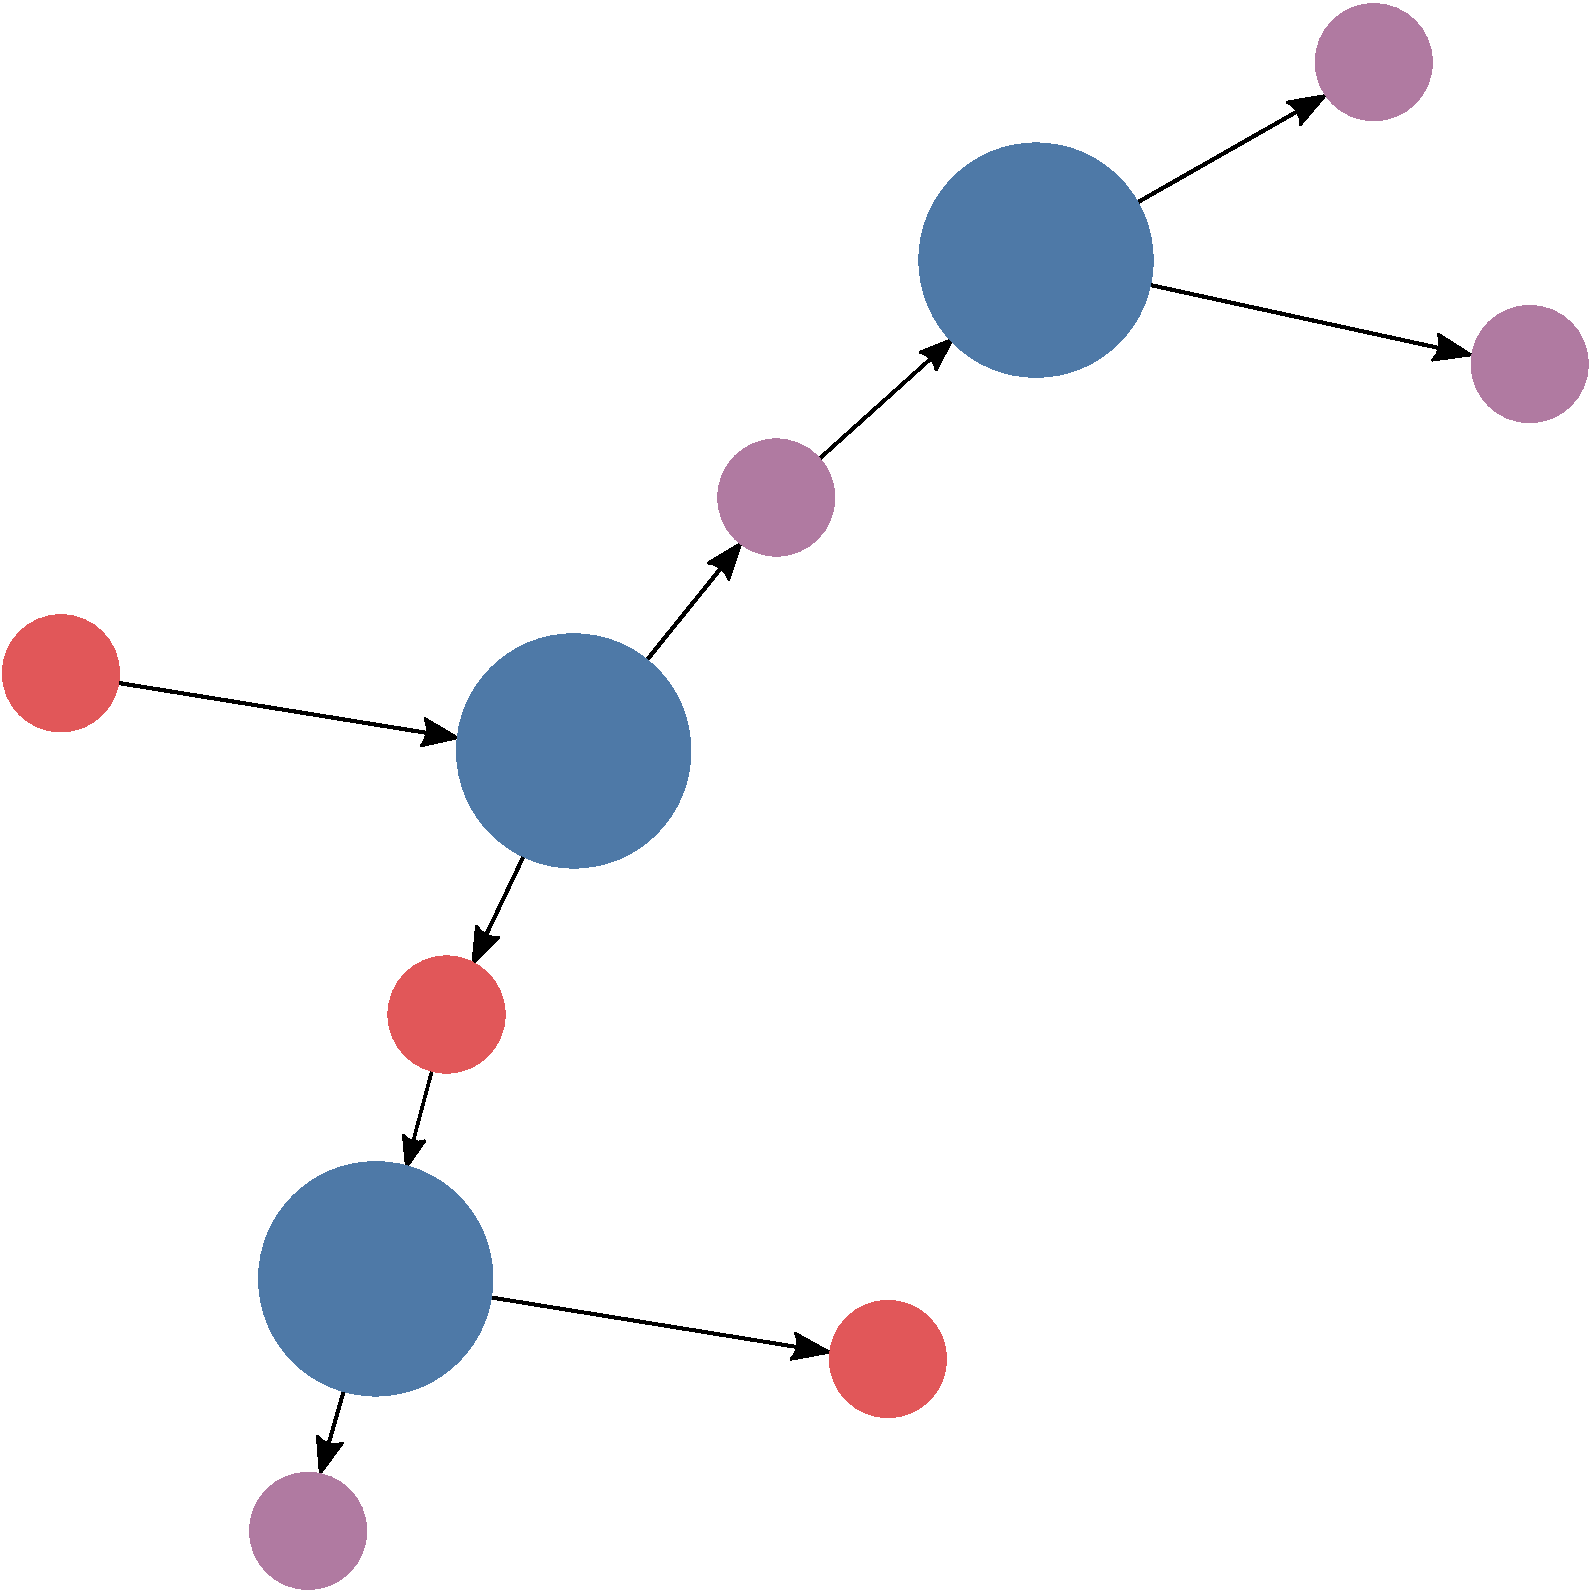
\includegraphics[width=\columnwidth]{figures/knn_simple_backward_think_2.pdf}
							\caption{Ply 3.}
						\end{subfigure}
						\caption{Backward thinking visualization in the KNN.}
					\end{figure}
				\end{block}
				\begin{block}{Conclusion}
					\begin{itemize}
						\item Skills learned:
						\begin{itemize}
							\item Planning and implementing large software project.
							\item Time management.
							\item People management.
						\end{itemize}
					
						\item Possible future work:
						\begin{itemize}
							\item Implement the missing NN and META layers.
							\item Explore further features in the KNN, such as learning and attention.
						\end{itemize}
					\end{itemize}
				\end{block}
			}
			\end{column}
		\end{columns}
	\end{frame}
\end{document}